\documentclass[12pt]{article}

%Preamble

\usepackage{amsmath}
\usepackage{amssymb}
\usepackage{amsthm}
\usepackage{amsrefs}
\usepackage{amsfonts}
%\usepackage{dsfont}
\usepackage{mathrsfs}
\usepackage{mathtools}
%\usepackage{stmaryrd}
%\usepackage[all]{xy}
\usepackage{enumerate}
\usepackage[shortlabels]{enumitem}
\usepackage{verbatim} %% includes comment environment
\usepackage{hyperref}
\usepackage[capitalize]{cleveref}
\crefformat{equation}{~(#2#1#3)}
\usepackage{caption, subcaption}
\usepackage{graphicx}
\graphicspath{{figures/}}
\usepackage{fullpage} %%smaller margins
\usepackage[all,arc]{xy}
\usepackage{mathrsfs}

%% Sectioning, Header / Footer, ToC
\usepackage{titlesec}
\usepackage{fancyhdr}
\usepackage{tocloft}


%% Optional Code Snippets

%\usepackage{minted} %Render Code.
%% Must add (% !TEX option = --shell-escape) to top of page.
%\usemintedstyle{colorful}

\hypersetup{
    linktoc=all,     %set to all if you want both sections and subsections linked
}

\newcommand{\bbF}{\mathbb{F}}
\newcommand{\bbN}{\mathbb{N}}
\newcommand{\bbQ}{\mathbb{Q}}
\newcommand{\bbR}{\mathbb{R}}
\newcommand{\bbZ}{\mathbb{Z}}
\newcommand{\bbC}{\mathbb{C}}
\newcommand{\calF}{\mathcal{F}}
\newcommand{\Prob}{\mathbb{P}}

\newcommand{\abs}[1]{ \left| #1 \right| }
\newcommand{\diff}[2]{\frac{d #1}{d #2}}
\newcommand{\infsum}[1]{\sum_{#1}^{\infty}}
\newcommand{\norm}[1]{ \left|\left| #1 \right|\right| }
\newcommand{\eval}[1]{ \left. #1 \right| }

\renewcommand{\phi}{\varphi}

%--------Theorem Environments--------
%theoremstyle{plain} --- default
\newtheorem{thm}{Theorem}[section]
\newtheorem{cor}[thm]{Corollary}
\newtheorem{prop}[thm]{Proposition}
\newtheorem{lem}[thm]{Lemma}
\newtheorem{conj}[thm]{Conjecture}
\newtheorem{quest}[thm]{Question}

\theoremstyle{definition}
\newtheorem{defn}[thm]{Definition}
\newtheorem{defns}[thm]{Definitions}
\newtheorem{con}[thm]{Construction}
\newtheorem{exmp}[thm]{Example}
\newtheorem{exmps}[thm]{Examples}
\newtheorem{notn}[thm]{Notation}
\newtheorem{notns}[thm]{Notations}
\newtheorem{addm}[thm]{Addendum}
\newtheorem{exer}[thm]{Exercise}

\theoremstyle{remark}
\newtheorem{rem}[thm]{Remark}
\newtheorem{rems}[thm]{Remarks}
\newtheorem{warn}[thm]{Warning}
\newtheorem{sch}[thm]{Scholium}

\numberwithin{equation}{section}

\bibliographystyle{plain}

%% Sectioning Aesthetics
\titleformat{\section}
{\normalfont\Large\bfseries}{\thesection.}{1em}{}
\titleformat{\subsection}
{\normalfont\Large\bfseries}{\thesubsection}{1em}{}
\titleformat{\subsubsection}
{\normalfont\normalsize\bfseries}{\thesubsubsection}{1em}{}
\titleformat{\paragraph}[runin]
{\normalfont\normalsize\bfseries}{\theparagraph}{1em}{}
\titleformat{\subparagraph}[runin]
{\normalfont\normalsize\bfseries}{\thesubparagraph}{1em}{}


%% Header Aesthetics
\pagestyle{fancy}

\setlength{\headheight}{16pt}
\setlength{\headsep}{0.3in}
\renewcommand{\headrulewidth}{0.4pt}
\renewcommand{\footrulewidth}{0.4pt}
\renewcommand{\contentsname}{\hfill\bfseries\Large Table of Contents\hfill}
\renewcommand{\sectionmark}[1]{\markright{ #1}}

\lhead{\textbf{}} % controls the left corner of the header
%\chead{\fancyplain{}{\rightmark }}
 % controls the center of the header / adds section # to top
\rhead[]{Marlin Figgins} % controls the right corner of the header
\lfoot{Last updated: \today} % controls the left corner of the footer
\cfoot{} % controls the center of the footer
\rfoot{Page~\thepage} % controls the right corner of the footer

\title{\bfseries\huge{AMATH 561A: Probability and Random Processes}\vspace{-1ex}} \author{\href{marlinfiggins@gmail.com}{\Large{Marlin Figgins}}\vspace{-2ex}}
\date{\large{Oct. 1, 2020}}

\begin{document}

\maketitle

	\section*{\hfill Introduction \hfill}

  This is a collection of my notes taken during AMATH 561A during fall quarter 2020 at the University of Washington.

  \thispagestyle{empty}

  %% Table of Contents Page/
  \newpage
  \tableofcontents
  \thispagestyle{empty}
  \newpage

  %% Set first page after ToC
  \setcounter{page}{1}

  %% Start here.

  \section{Probability Spaces and Random Variables}%
  \label{sec:probability_spaces_and_random_variables}
  %TODO: Port over some of old notes / blog post figures introducing the study of probability.

  % We'll begin with a slightly informal definition of a probability space. 

  \begin{defn}[Probability Space: Version A]
    A \emph{probability space} is a triple $(\Omega, \calF, \Prob)$ where $\Omega$ is the \emph{sample space} or the space of possible outcomes, $\calF$ is the set of events which are subsets of $\Omega$ and $\Prob \colon \calF \to [0,1]$ is a probability measure that assigns probabilities to events.
 \end{defn} 

 \begin{exmp}[Rolling a fair standard die]
 In this case, we have six possible outcomes as our die is six-sided. Therefore, our sample space is 

 \begin{equation}
   \Omega = \{ 1, 2, 3, 4, 5, 6 \}.
 \end{equation}

 The set of events in this case are all possible subsets of $\Omega$ i.e. the power set $\mathcal{P}(\Omega)$. Finally, since we specificed that the die is fair, each outcome is equally likely, so our probability measure $\Prob$ is uniform over $\Omega$. Therefore, our probability of a given event is just the fraction of our possible out comes which are in the event.

 \begin{equation}
 \Prob(A) = \frac{\abs{A}}{\abs{\Omega}} = \frac{\abs{A}}{6} \text{ for all  } A \in \calF.
 \end{equation}

 For example, we would say that the probability of rolling an even number would be given by

 \begin{equation}
   \Prob(\{ 2, 4, 6 \}) = \frac{3}{6} = 0.5.
 \end{equation}
 \end{exmp}

 In this example, it is simple enough to use all possible subets are our set of events, but as we attempt to deal with more complicated probability spaces, we'll need to develop a more rigorous notion of what constitutes an event, so that our probability measures will have certain properties of interest. This idea is formalized by the $\sigma$-algebra.

 \begin{defn}[$\sigma$-algebra]
   A non-empty collection of subsets of $\Omega$ is a \emph{$\sigma$-algebra} of $\Omega$ if it satistifies the following:

 \begin{enumerate}[(i)]
   \item For each event $A\in \calF$, then its complement $A^c\in \calF$
   \item If we have a countable sequence of sets $A_i \in \calF$, then their union $\bigcup_i A_i \in \calF$.
 \end{enumerate}

 These two conditions form the statement that a $\sigma$-algebra is closed under complements and countable unions.
 \end{defn}

 \begin{prop}
 The definition of the $\sigma$-algebra implies that $\sigma$-algebras are also closed under countable intersection because
 \begin{equation}
   \bigcap_i A_i = \left( \bigcup_i A_i^c \right)^c.
 \end{equation}
 \end{prop}

Minimally, we know that a $\sigma$-algebra must contain the empty set and the space on which it lives. 

\begin{exer}
   Show that any $\sigma$-algebra of $\Omega$ contains both the entire space $\Omega$ and the empty set.
\end{exer}

This formalizes the notion of events and combinations of events espressed earlier. Now, we'll develop a formal notion of probabiltiy usinng measure theory.

%TODO: Clean this up and perhaps limit to probability measures.
 When we have a probability space $\Omega$ and a $\sigma$-algebra $\calF$ on $\Omega$, we can define a measure on the space $(\Omega, \calF)$. \emph{Describe what a measure is intuitively.}

 \begin{defn}[Measure]
   A \emph{measure} is a function $\mu: \calF \to [0, \infty)$ which satisfies:
   \begin{enumerate}[(i)]
     \item $\mu(A) \geq \mu(\emptyset) = 0$ for all $A\in\calF$
     \item if $A_i \in F$ is a countable sequence of disjoint sets, then 
       \begin{equation}
         \mu\left(\bigcup_i A_i \right) = \sum_i \mu(A_i).
       \end{equation}
   \end{enumerate}
   In the case that $\mu(\Omega)$, we will call $\mu$ a \emph{probability measure} and denote it as $\Prob$.
 \end{defn}

 \begin{figure}[ht]
   \centering
   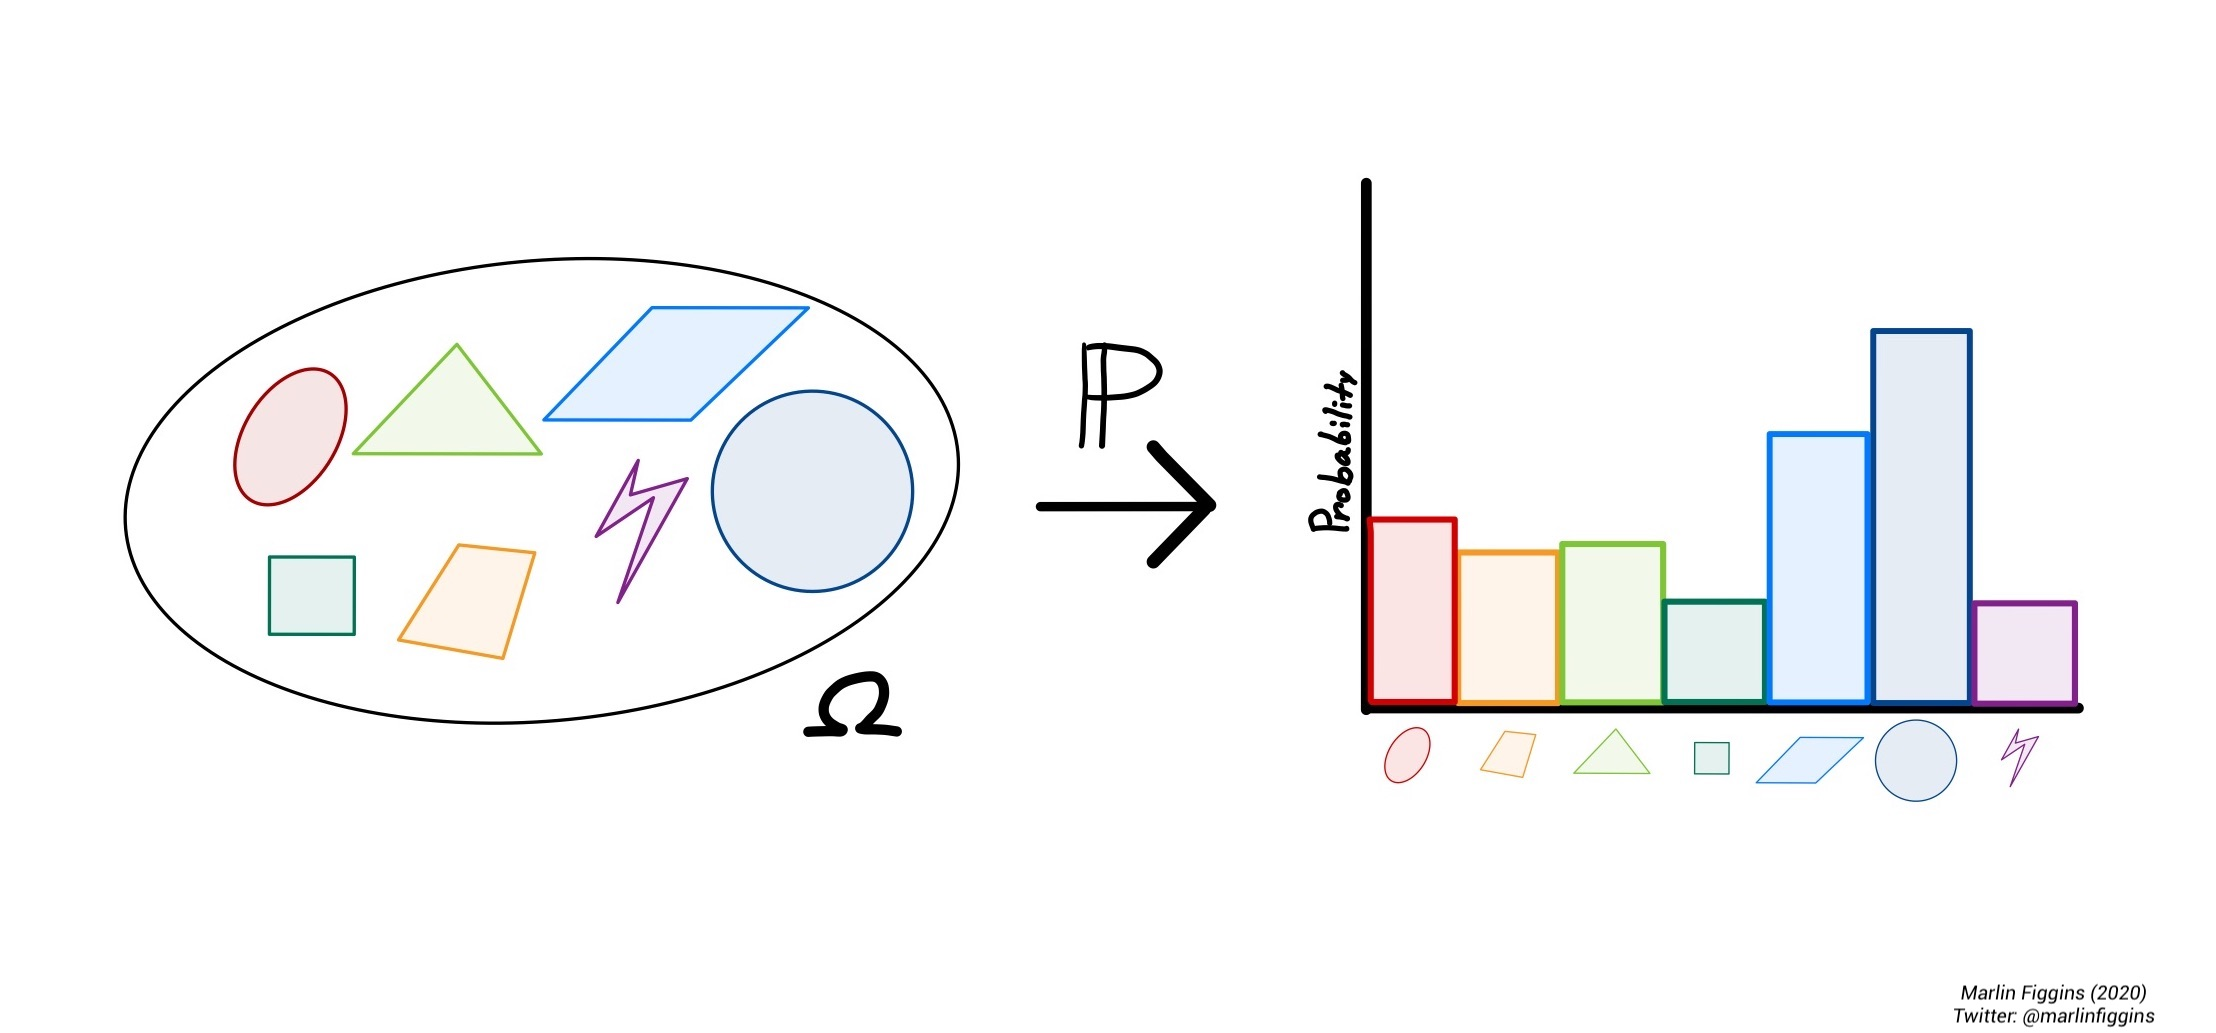
\includegraphics[width=0.9\linewidth]{intro-to-prob-measure.jpg}
   \caption{A probability measure $\Prob$ takes measurable subsets $E\in \calF$ to a numerical value in $[0,1]$.}%
   \label{fig:intro-to-prob-measure}
 \end{figure}

 Our definition of measure allows us to ensure that our notion of probabilty satisifies some of the intuitive properties one might expect of probabilities.

 \begin{thm}[Properties of measure]\leavevmode
   \begin{enumerate}[(i)]
     \item \emph{Monotonicity.} If $A\subset B$, then $\mu(A) \leq  \mu(B)$.
   \item \emph{Subadditivity.} If $A\subset \bigcup_{j\in\bbN} A_j$, then 
        \begin{equation}
        \mu(A) \leq \sum_{j\in\bbN} \mu(A_m).
        \end{equation}
 \end{enumerate}
 \end{thm}

 \begin{proof}[Proof of monotonicity]
   Finish proof. 
 \end{proof}

 \begin{proof}[Proof of subadditivity]
  Finish proof. 
 \end{proof}
 
 \begin{figure}[ht]
   \centering
   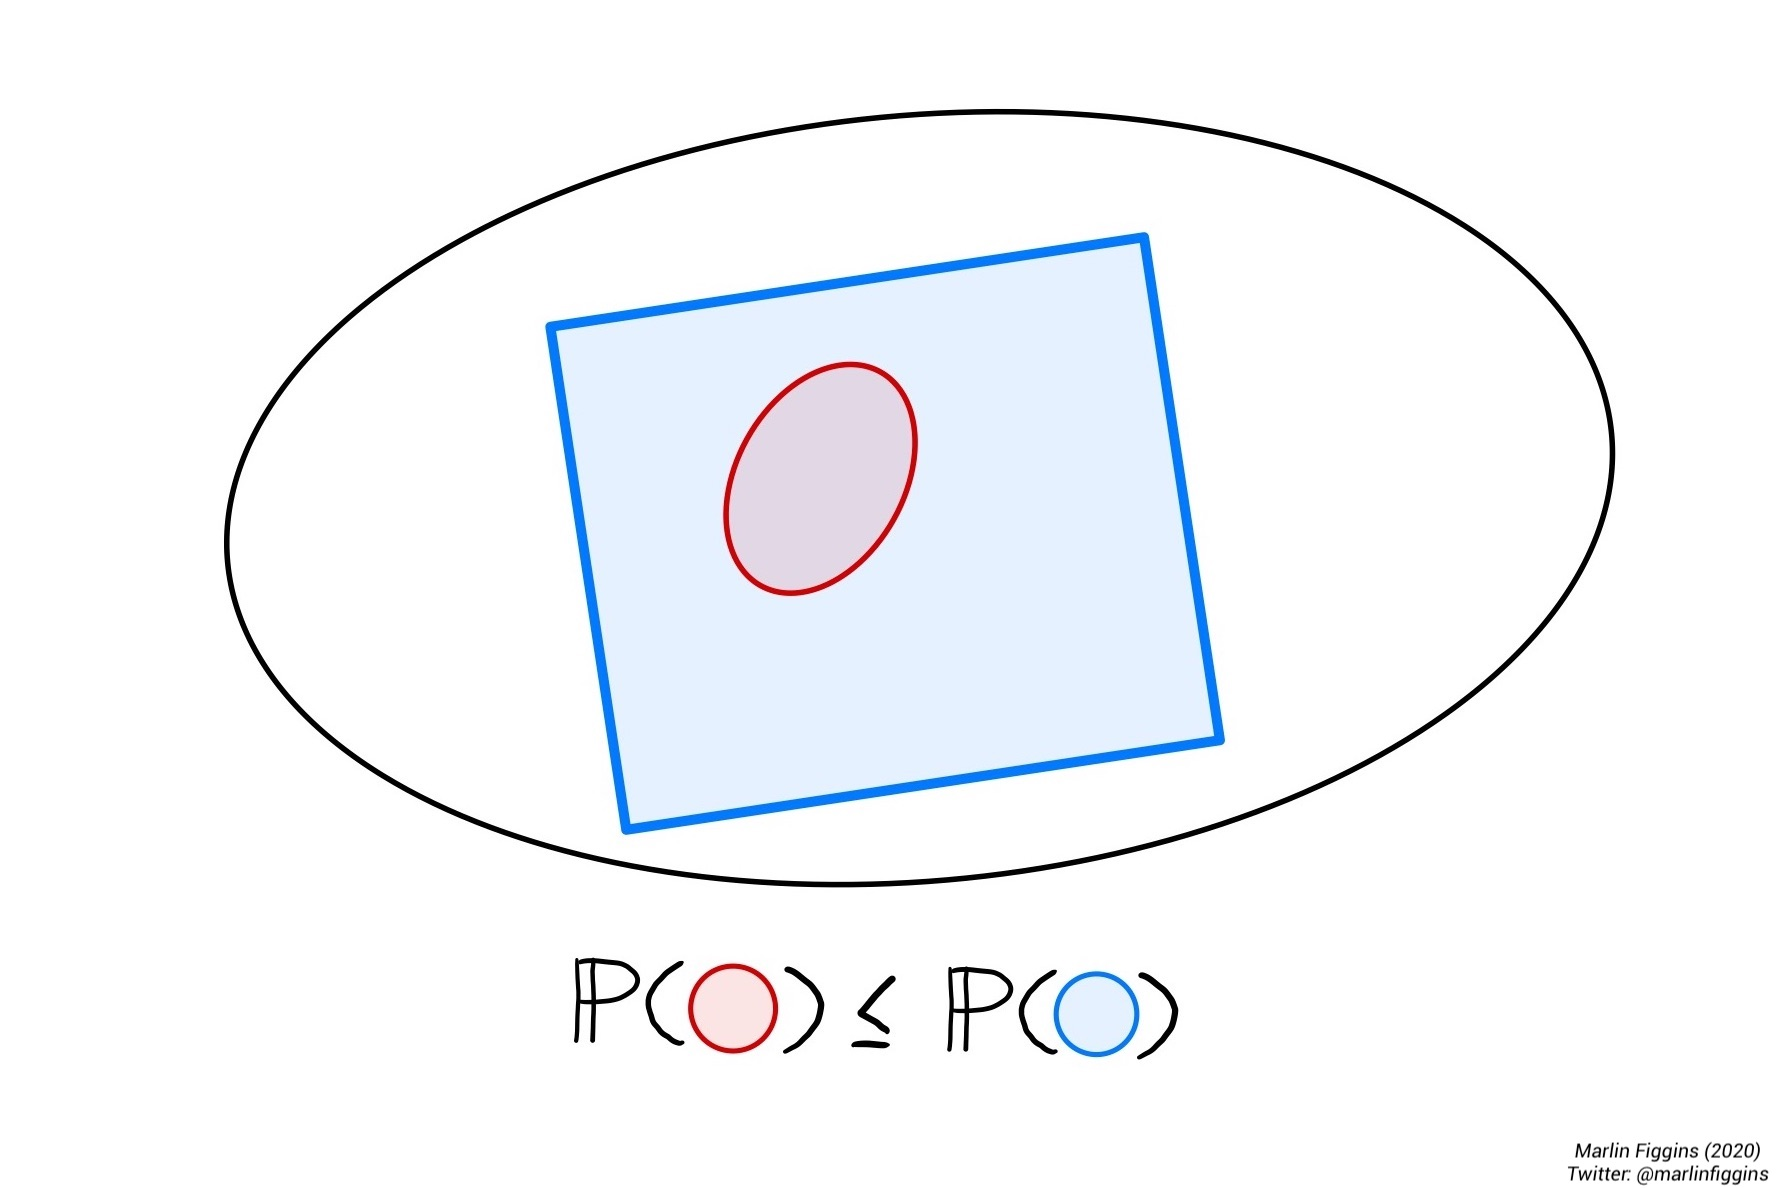
\includegraphics[width=0.6\linewidth]{intro-to-prob-subset-ineq.jpg}
   \caption{If a probability measure is consistent with our formulation, it ought to be monotonic. Appending additional outcomes to an event $E$ should never decrease its probability of occuring. }%
   \label{fig:intro-to-prob-subset-ineq}
 \end{figure}

 % TODO: Exposition about the fact that we can pass to limits
 \begin{thm}[Continuity of measure]\leavevmode
   \begin{enumerate}[(i)]
     \item \emph{Continuity from above.} If we have a sequence of increasing subsets $A_1 \subset A_2 \subset \cdots $ such that $\bigcup_i A_i = A$, then 
       \begin{equation}
         \mu(A_i) \uparrow \mu(A) \text{ as } i \to \infty.
       \end{equation}
     \item \emph{Continuity from below.} If we have a sequence of decreasing subsets $A_1 \supset A_2 \supset \cdots $ such that $\bigcup_i A_i = A$, then 
       \begin{equation}
         \mu(A_i) \downarrow \mu(A) \text{ as } i \to \infty. 
       \end{equation}
 \end{enumerate}
 \end{thm}

 \begin{exer}
   Prove that in a probability space $(\Omega, \calF, \Prob)$ 
   \begin{equation} 
     \Prob(A) = 1 - \Prob(A^c) \text{ for any event } A \in \cal F.
   \end{equation}
 \end{exer}

\subsection{Discrete Probability Spaces}%
\label{sub:discrete_probability_spaces}

\paragraph{Constructing a discrete probability space.}

We'll now focus on the case of discrete probability spaces. Let $\Omega$ be a countable set. That is, either finite or countably infinite. Also, let $\calF$ be the set of all subsets of $\Omega$ which we will call the power set $\mathcal{P}(\Omega)$. We can know endow $(\Omega, \calF)$ with a probability measure. 

\begin{thm}
  Suppose we have a countable set $\Omega$ with a $\sigma$-algebra $\calF=\mathcal{P}(\Omega)$. Then any function $p \colon \Omega \to [0, 1]$ such that 
\begin{equation}
  \sum_{\omega\in\Omega} p(\omega) = 1
\end{equation}
induces a probability measure $\Prob$ on $(\Omega, \calF)$ as follows. For any event $A\in \calF$, we define the probability of $A$ as 
\begin{equation}
  \Prob(A) = \sum_{\omega \in A} p(\omega).
\end{equation}
We call the function $p$ the \emph{probability mass function} of $\Prob$.
\end{thm}

\begin{exmp}[Repeated fair coins]
Consider the following experiment: We have a fair coin and we flip it until it lands on heads. We can write the possible outcomes as sequences of heads and tails, so that
\begin{equation}
  \Omega = \{ H, TH, TTH, TTH, \ldots \}.
\end{equation}

As before, we can let $\calF = \mathcal{P}(\Omega)$. Let's motivate our choice of probability mass function $p$. Assuming that the probability of heads and tails at every flip is $\frac{1}{2}$, then we have a probability of $\left(\frac{1}{2}\right)^n$ for having $n$ consequective flips. This tells us that
\begin{equation}
p(\underbrace{T\cdots T}_{n \text{ tails}} H) = \left(\frac{1}{2}\right)^n.
\end{equation}

We can check that this indeed sums to one:

\begin{equation}
  \sum_{\omega\in\Omega}p(\omega) = \sum_{i=1}^{\infty} \left(\frac{1}{2}\right)^n. 
\end{equation}

As shown above, this probability mass function induces a probability measure $\Prob$ on $(\Omega, \calF)$. We can now use this measure the compute the probability of events like:

\begin{align}
  A &= \{ \text{Heads appears before third toss.} \} = \{H, TH \},\\
  B &= \{ \text{There are an even number of tails.}\} = \{H, TTH, TTTTH, \ldots\}.
\end{align}

We can then compute these probabilities as:
\begin{align}
  \Prob(A) &= \frac{1}{2} + \frac{1}{4}, \\
  \Prob(B) &= \frac{1}{2} + \frac{1}{2^3} + \frac{1}{2^5} + \cdots = \frac{2}{3}.   
\end{align}
\end{exmp}

%TODO: Add text saying asking what would happen if we wanted to pass to ask about the long-term behavior of the coin-tossing experiment. What if we wanted to flip an infinite number of coins...

\subsection{Uncountable probability spaces}%
\label{sub:uncountable_probability_spaces}

%TODO: Add text stating that we can't simply use the the power set of uncountable sets to generate a $\sigma$-algebra.

We'll begin by further describing $\sigma$-algebra, so that we can understand what an uncountable $\sigma$-algebra must satisft. %TODO: Edit this slightly

\begin{prop}
  \emph{The intersection of $\sigma$-algebras is again a $\sigma$-algebra.} Let $I \neq \emptyset$ be an arbitrary set. If we have a collection of $\sigma$-algebras $\calF_i$ for $i\in I$ defined on $\Omega$, then their intersection 

  \begin{equation}
    \bigcap_{i\in I} \calF_i \text{ is a $\sigma$-algebra on } \Omega. 
  \end{equation}
\end{prop}

\begin{proof}
  Per an earlier exercise, all $\sigma$-algebras in the collection $\calF_i$ must contain $\emptyset$ and $\Omega$. Therefore, these sets are also in the intersection. For any event $A$ that is in every $\calF_i$, $A^c$ must be in $\calF_i$ since they are closed under complements. A similar argument holds for countable collections of events $A_j$ and their unions.
\end{proof}

Thus, if we are given a sample space $\Omega$ and $\mathcal{A}$ a collection of subsets of $\Omega$, then there is a smallest $\sigma$-algebra which contains $\mathcal{A}$. 

\begin{defn}[$\sigma$-algebra generated by $\mathcal{A}$]
  Given a sample space $\Omega$ and a collection of its subsets $\mathcal{A}$, the $\sigma$-algebra generated by $\cal{A}$ is the smallest $\sigma$-algebra containing $\mathcal{A}$. We denote this as $\sigma(\mathcal{A})$. 
\end{defn}

\begin{exmp}
  Given $\Omega = \{ 1,2,3,4 \}$ and $\mathcal{A} = \{ \{1\}. \{1,2\} \}$, the smallest $\sigma$-algebra containing $\mathcal{A}$ is
  \begin{equation}
    \sigma{\mathcal{A}} = \{\emptyset, \Omega, \{1\}, \{2,3,4\}, \{1,2\},\{3,4\},\{1,3,4\},\{2\}\}    
  \end{equation}
\end{exmp}

\paragraph{Constructing uncountable probability spaces}%
\label{par:constructing_uncountable_probability_spaces}

Let's consider the experiment of drawing a random number between $[0,1]$. In this case, our sample space is clearly $\Omega = [0,1]$. In this case, we would like each number to be equally likely, but we can't simply set each number to occur with probability $\Prob(A) = \frac{\abs{A}}{\abs{\Omega}}$ as with the case of the fair die because our space is uncountable! Ideally, we want to find some function $p(x)=p$ which describes the probability that we choose $x\in[0,1]$. What is the probabiltiy that our chosen number is rational (in $\bbQ$). By the countable additivity of our probability measure, 

\begin{align}
  \Prob(\bbQ \cap [0,1]) &= \Prob( \bigcup_{ x\in \bbQ\cap[0,1]} \{x\}) \\ 
                         &= \sum_{x\in Q\cap[0,1]} p(x) = \sum_{x\in Q\cap[0,1]} p. 
\end{align}

For any positive real value of $p$, the rightmost sum is infinite which is nonsensical as the probability of any event cannot exceed one. Thus the probability of an single value must be exactly 0. By the countable additivity of measure, this means that any countable subset of $[0,1]$ must have probablity 0.

\paragraph{The Lebesgue measure on $[0,1]$} We'll try an alternative approach to constructing probability spaces. We begin by defining the probabilities of certain subsets of interest and we extend this to the $\sigma$-algebra containing that collection of subsets. For example, we can specify that the probability of choosing a number between $a$ and $b$ is 

\begin{equation}
  \Prob((a,b]) = b - a \text{ for $a$ and $b$ with } 0\leq a < b \leq 1.
\end{equation}

This is a uniform probability measure on $[0,1]$ and it is called the \emph{Lebesgue measure on $[0,1]$}.

\paragraph{Borel $\sigma$-algebra}%
\label{par:borel_sigma_algebra}

We can extend the Lebesgue measure described below by extending it to the $\sigma$-algebra generated by intervals of the form $(a,b]$ by using the countable additivity property of measures. This is called the \emph{Borel $\sigma$-algebra} on $[0,1]$ is denoted by $\mathcal{B}([0,1])$. $\mathcal{B}([0,1])$ is the smallest $\sigma$-algebra containing all open sets in $[0,1]$. Additionally, the extension of our measure to the Borel $\sigma$-algebra is unique by the Caratheodory Extension theorem. That being said, the Lebesgue measure cannot be extended to all subsets of $[0,1]$. That being said, we will restrict our attention to study $([0,1], \mathcal{B}([0,1]))$. 

\begin{exmp}[Infinite coin tosses]
  Suppose that we conduct an infinite sequence of coin tosses. Let the probability of each coin showing heads be $p$ and the probability of tails be $q=1-p$. In this case, our sample space is all possible countable sequences of heads and tails. There is a one-to-one correspondence between $\Omega$ and $[0,1]$ by considering the base two expansion of numbers between $[0,1]$. As $\Omega$ is uncountable, we begin by specifying the probability on some reasonable subset of events which we can expand to some larger $\sigma$-algebra. We'll represent $w\in\Omega$ as a sequence $\omega_1\omega_2\ldots$ where each $w_i$ is the result of the $i$th coin toss. Let $A_H = \{ \omega\in\Omega\mid \omega_1 = H \}$.  That is, $A_H$ is the event that the first coin toss is heads. Naturally, the probability of $A_H$ should be the probability of flipping heads, so that

  \begin{equation}
    \Prob(A_H) = p \text{ and similarly } \Prob(A_T) = q = 1 - p.
  \end{equation}
  These events generate a $\sigma$-algebra $\calF_1 = \sigma(\{A_H, A_T \})$. In fact, we can define a series of $\sigma$-algebras $\calF_n$ based on the events of the first $n$ coin tosses. For example, consider $\calF_2$. This would contain events like:
\begin{align}
A_{HH} = \{\omega\in\Omega \mid \omega_1 = H, \omega_2 = H\}, &\quad A_{HT} = \{\omega\in\Omega \mid \omega_1 = H, \omega_2 = T\}, \\
A_{TH}= \{\omega\in\Omega \mid \omega_1 = T, \omega_2 = H\}, &\quad A_{TT}= \{\omega\in\Omega \mid \omega_1 = T, \omega_2 = T\}.
\end{align}

These events would have probabilities:
\begin{align}
  \Prob(A_{HH}) = p^2, &\quad \Prob(A_{HT}) = pq, \\
  \Prob(A_{TH}) = pq, &\quad \Prob(A_{TT}) = q^2.
\end{align}

We can similarly extend this to the events in $\calF_n$. Due to our construction, we have an increasing sequence of $\sigma$-algebras $\calF_1 \subset \calF_2 \subset \calF_3 \ldots$ which describe the results of finite coin tosses. We'll then define $\calF_\infty = \cup_{n\in\bbN} \calF_n$. This is \textbf{not} a $\sigma$-algebra because it is not closed under countable intersection. Consider the event $w_H$ which is the infinite sequence of outcomes with all $H$. We also consider the outcomes $\omega_{nH}$ which is where we count $n$ heads in a row. As you can see,
\begin{equation}  
  \{\omega_H \} = \bigcap_{n\in\bbN} \{\omega_{mH}\}.
\end{equation}
However,$ \{ w_H\}$ is not in $\calF_n$ for any $n$ since it depends on the results of all coin tosses. This means that $\calF_\infty$ cannot be a $\sigma$-algebra as it does not contain the countable union of $\{ \omega_{nH}\mid n\in\bbN\} \in \calF_\infty$. To remedy this, we can just use $\calF = \sigma(\calF_\infty)$. Once again, we can extend our probabilities to events in $\calF$ that are in $\calF_\infty$ uniquely. Unlike $\calF_\infty$, $\calF$ contains events which cannot be specified by any finite number of coin tosses like $\omega_H$ which we discussed before. We can assign a probability to this event using the continuity of measure from above. Since $\{\omega_{nH}\} \supset \{\omega_{(n+1)H}\}$ and $\{\omega_H \} = \cap_{n\in\bbN} \{\omega_{mH}\}$, it follows that 
\begin{equation}
  \Prob(\{\omega_{nH} \}) = p^n \downarrow P(\{\omega_H\}) = 0.
\end{equation}
\end{exmp}

\section{Independence, Martingales, and Conditioning}%
  \label{sec:independence_martingales_and_conditioning}
 
  \section{Characteristic Functions}%
  \label{sec:characteristic_functions}
  
  \section{Markov Chains}%
  \label{sec:markov_chains}
  
  \section{Generating Functions and Branching Processes}%
  \label{sec:generating_functions_and_branching_processes}
  
  \section{Convergence of Random Variables}%
  \label{sec:convergence_of_random_variables} 

\end{document}
